\documentclass[compress,pdf,mathserif]{beamer}
\usetheme{chpc}
\usepackage{tikz}
\usepackage{epstopdf}
\usepackage{ulem}
\usepackage{movie15}
\usepackage{amsmath}
\usepackage{mathabx}
\usepackage{xcolor}
\usepackage{algorithm,algorithmic}
\usepackage{pgfplots}

\title{Comparison of discrete fiber and asymptotic homogenization methods for modeling of fiber-reinforced materials deformations}
\author{\textit{Petr Zakharov}\\Petr Sivtsev}
\institute{SCTEMM 2019}
\date{June 19 - 21}

\renewcommand{\arraystretch}{1.5}

\begin{document}

\maketitle

\subsection{Content}
\begin{frame}
\begin{enumerate}
\item Introduction
\item Model problem
\item Approximations
\item Numerical simulations
\item Conclusion
\end{enumerate}
\end{frame}

\section{Introduction}
\subsection{Introduction}
\begin{frame}
    \begin{itemize}
        \item Fiber-reinforced materials are recommended as most of the strongest composite materials
        \item Numerical modeling of fiber-reinforced materials leads to huge grid size due to fiber size and count
        \item Discrete fiber method (discerte fracture method): one dimensional fibers
        \item Asymptotic homogenization method: averaged coarse problem
    \end{itemize}
\end{frame}

\section{Model problem}
\subsection{Model problem}
\begin{frame}
    \centering
    \begin{tikzpicture}[scale=1]
        \draw[gray] (0, 0) grid (4, 4);
        \draw (0, 0) rectangle (4, 4);
        \node at (2, -0.5) {$\Omega = \Omega_1 \cup \Omega_2$};
        \foreach \i in {1,...,4} {
            \foreach \j in {1,...,4} {
                \foreach \k in {1,...,4} {
                    \draw (\i-0.75, \j-\k/4+1/8)--(\i-0.25, \j-\k/4+1/8);
                }
            }
        }
        %\draw (3.5, 1.5) circle (0.75);
        \draw[->] (3.5, 1.5)--(8, 2);

        \draw[gray] (6, 0) rectangle (10, 4);
        \node at (8, -0.5) {$\Omega_2 = \bigcup_{i=1}^K \phi_i$};
        \foreach \k in {1,...,4} {
            \draw (7, \k-0.55) rectangle (9, \k-0.45);
            \node at (9.5, 4.5-\k) {$\phi_{i+\k}$};
        }
    \end{tikzpicture}

\begin{itemize}
\item    $\Omega_1$ is the main material
\item    $\Omega_2$ is the fibers
\end{itemize}
\end{frame}


\subsection{Stress-strain state}
\begin{frame}
\[
    \nabla \cdot \bm{\sigma} = \bm{f}, \quad \bm{x} \in \Omega,
\]

\begin{itemize}
    \item $\bm{\sigma}=\bm{C}\bm{\varepsilon}$ is the stress tensor
    \item $\bm{C}$ is the elastic tensor
    \item $\bm{\varepsilon}$ is the strain tensor
    \item $\bm{f}$ is the force source
\end{itemize}
\end{frame}

\subsection{Voight notation}
\begin{frame}
    \centering
    Stress and elastic tensors 
    \[
        \bm{\sigma} = \left(
        \begin{matrix}\sigma_{11}\\ \sigma_{22}\\ \sigma_{12}\end{matrix}
        \right), \quad
        \bm{C} = \left( \begin{matrix}
        C_{1111} & C_{1122} & C_{1112}  \\
        C_{2211} & C_{2222} & C_{2212}  \\
        C_{1211} & C_{1222} & C_{1212}  
        \end{matrix}  \right)
    \]

    Strain tensor
    \[
        \bm{\varepsilon} = \left(
        \begin{matrix}\varepsilon_{11}\\ \varepsilon_{22}\\ 2\, \varepsilon_{12}\end{matrix}
        \right) = \left( \begin{matrix}\frac{\partial u_1}{\partial x_1}\\ \frac{\partial u_2}{\partial x_2} \\ \frac{\partial u_2}{\partial x_1} + \frac{\partial u_1}{\partial x_2} \end{matrix} \right).
    \]
\end{frame}

\subsection{Lame parameters}
\begin{frame}
    \centering
    Isotropic materials elastic tensor
    \[
    \bm{C}_i = \left( \begin{matrix}
    \lambda_i+2\mu_i & \lambda_i & 0  \\
    \lambda_i & \lambda_i+2\mu_i & 0  \\
    0 & 0 & \mu_i 
    \end{matrix}  \right), \quad \bm{x} \in \Omega_i, \quad i=1,2.
    \]
    \[
    \lambda_i = \frac{E_i\, \nu_i}{(1 + \nu_i) (1 - 2 \nu_i)}, \quad
    \mu_i = \frac{E_i}{2 (1 + \nu_i)}, \quad \bm{x} \in \Omega_i, \quad i=1,2.
    \]
    \begin{itemize}
        \item $E_i$ is the Young modulus
        \item $\nu_i$ is the Poisson coefficient
    \end{itemize}
\end{frame}

\subsection{Boundary conditions}
\begin{frame}
    \centering
    \begin{tikzpicture}[scale=0.75]
        \draw[gray] (0, 0) grid (4, 4);
        \draw (0, 0) rectangle (4, 4);
        \foreach \i in {1,...,4} {
            \foreach \j in {1,...,4} {
                \foreach \k in {1,...,4} {
                    \draw (\i-0.75, \j-\k/4+1/8)--(\i-0.25, \j-\k/4+1/8);
                }
                \draw (-0.2, \j-\i/4+1/8)--(0.0, \j-\i/4+1/4);
            }
        }
        \draw[ultra thick] (0,0)--(0,4);
        \node at (-0.5, 2) {$\Gamma_L$};
        \node at (4.5, 2) {$\Gamma_R$};
    \end{tikzpicture}

    Dirichlet condition on the left border
    \[
    \bm{u} = (0, 0), \quad \bm{x} \in \Gamma_L.
    \]
    Neumann condition on the right border
    \[
    \bm{\sigma}_{\bm{n}} = \bm{g}, \quad \bm{x} \in \Gamma_R.
    \]
    $\bm{\sigma}_{\bm{n}}=\bm{\sigma}\,\bm{n}$ and $\bm{n}$ is the normal vector to the border
\end{frame}

\section{Approximations}
\subsection{Finite element approximation}
\begin{frame}
    \centering
    Bilinear form
    \[
        a(\bm{u}, \bm{v}) = \int_{\Omega_1} \bm{C}_1 \, \bm{\varepsilon}(\bm{u}): \bm{\varepsilon}(\bm{v})\, {\rm d}\bm{x} + \int_{\Omega_2} \bm{C}_2 \, \bm{\varepsilon}(\bm{u}) : \bm{\varepsilon}(\bm{v}) \,{\rm d}\bm{x},
    \]
    Linear form
    \[
        L(\bm{v}) = \int_{\Omega}\bm{f}\, \bm{v}\, {\rm d}\bm{x} + \int_{\Gamma_R}\bm{g}\, \bm{v}\, {\rm d}\bm{s},
    \]
    Trial and test function spaces
    \[
        V = \widehat{V} = \{\bm{v} \in H^1(\Omega) : \bm{v} = (0, 0), \bm{x} \in \Gamma_L \},
    \]

    $H^1$ is the Sobolev function space
\end{frame}

\subsection{Discrete fiber approximation}
\begin{frame}
    \centering
    \begin{tikzpicture}[scale=0.75]
        \draw[gray] (5, 0) rectangle (9, 4);
        \foreach \k in {1,...,4} {
            \draw (6, \k-0.55) rectangle (8, \k-0.45);
            \node at (8.5, 4.5-\k) {$\phi_\k$};
        }
        \node at (7, -1) {$\Omega_2=\bigcup_{i=1}^K \phi_i$};
        \draw[->](9.5, 2)--(11.5,2);
        \draw[gray] (12, 0) rectangle (16, 4);
        \foreach \k in {1,...,4} {
            \draw (13, \k-0.5) -- (15, \k-0.5);
            \node at (15.5, 4.5-\k) {$\gamma_\k$};
        }
        \node at (14, -1) {$\Gamma_2=\bigcup_{i=1}^K \gamma_i$};
    \end{tikzpicture}

\end{frame}

\subsection{Discrete fiber approximation (2D)}
\begin{frame}
    \centering
    Bilinear form
    \[
        \begin{gathered}
a(\bm{u}, \bm{v}) = \int_\Omega \bm{C}_1\, \bm{\varepsilon}(\bm{u}) : \bm\varepsilon(\bm{v})\, {\rm d}\bm{x}+\\
\int_{\Gamma_{2}} d\, (\lambda_2 + 2\mu_2 - \lambda_1 - 2\mu_1) (\nabla \bm{u}_{\bm{\tau}}\, {\bm{\tau}})(\nabla \bm{v}_{\bm{\tau}}\, {\bm{\tau}}) {\rm d}\bm{s},
        \end{gathered}
\]
Linear form
\[
L(\bm v) = \int_{\Omega}\bm{f}\, \bm{v}\, {\rm d}\bm{x} +\int_{\Gamma_R}\bm{g}\, \bm{v}\, {\rm{d}}\bm{x},
\]

\begin{itemize}
    \item $d$ is thickness of fibers
    \item $\bm{u}_{\bm{\tau}} = \bm{u}\, \bm{\tau}$ and $\bm{\tau}$ is the tangent vector to a fiber line
    \item Function spaces same as in FEM
\end{itemize}
\end{frame}

\subsection{Asymptotic homogenization approximation}
\begin{frame}
    \centering
    \begin{tikzpicture}[scale=0.75]
        \draw[gray] (5, 0) rectangle (9, 4);
        \foreach \k in {1,...,4} {
            \draw (6, \k-0.55) rectangle (8, \k-0.45);
        }
        \node at (7, -1) {$\bm{C}_i, i=1,2$};
        \draw[->](9.5, 2)--(11.5,2);
        \draw[gray] (12, 0) rectangle (16, 4);
        \node at (14, -1) {$\bm{C}^*$};
    \end{tikzpicture}
    
    \centering
    \vspace{1em}
    $\bm{C}^*$ is the effective elastic tensor
\end{frame}

\subsection{Asymptotic homogenization approximation}
\begin{frame}
\centering
Average of the stress tensor
\[
\langle \bm{\sigma} \rangle = \langle \bm{C}\, \bm{\varepsilon} \rangle = \bm{C}^* \langle \bm{\varepsilon}\rangle,
\]

Average
\[
\langle\psi\rangle = \frac{\int_\omega \psi \, {\rm d}\bm{x}}{\int_\omega \, {\rm d}\bm{x}},
\]

$\omega$ is a periodic domain.
\end{frame}

\subsection{Periodic problems}
\begin{frame}
    \centering
    $\bm{u}^k$ is the solution with $\bm{f}^k, k=1,2,3$
    \begin{itemize}
        \item $\bm{f}^1 = -\nabla \cdot \bm{C}\, \bm{\varepsilon}((x_1, 0))$,
        \item $\bm{f}^2 = -\nabla \cdot \bm{C}\, \bm{\varepsilon}((0, x_2))$,
        \item $\bm{f}^3 = -\nabla \cdot \bm{C}\, \bm{\varepsilon}((x_2/2, x_1/2))$.
    \end{itemize}
\vspace{1em}

    The effective elastic tensor
    \begin{itemize}
        \item $C^*_{ij11} = \langle \sigma_{ij}^1 \rangle, \quad ij=11, 22, 12$,
        \item $C^*_{ij22} = \langle \sigma_{ij}^2 \rangle, \quad ij=11, 22, 12$,
        \item $C^*_{ij12} = \langle \sigma_{ij}^3 \rangle, \quad ij=11, 22, 12$.
    \end{itemize}

    $\bm{\sigma}^k=\bm{C}\bm{\varepsilon}(\bm{u}^k),\quad k=1,2,3$
\end{frame}

\subsection{Coarse problem}
\begin{frame}
    \centering
    Bilinear form
    \[
a(\bm{u}, \bm{v}) = \int_\Omega \bm{C}^* \, \bm{\varepsilon}(\bm{u}) : \bm{\varepsilon}(\bm{v})\, {\rm d}\bm{x}\]
Linear form
\[
L(\bm{v}) = \int_\Omega \bm{f}\, \bm{v} \, {\rm d}\bm{x} + \int_{\Gamma_R} \bm{g}\, \bm{v}\, {\rm d}\bm{s}.
\]

We don't compute a higher order solution of the asymptotic homogenization method
\end{frame}

\section{Numerical simulations}
\subsection{Numerical simulations}
\begin{frame}
    \centering
    \begin{tikzpicture}[scale=0.75]
        \draw[gray] (0, 0) grid (4, 4);
        \draw (0, 0) rectangle (4, 4);
        \foreach \i in {1,...,4} {
            \foreach \j in {1,...,4} {
                \foreach \k in {1,...,4} {
                    \draw (\i-0.75, \j-\k/4+1/8)--(\i-0.25, \j-\k/4+1/8);
                }
            }
        }
    \end{tikzpicture}
    \vspace{1em}

    \begin{itemize}
        \item $\Omega$ contains $n \times n$ equal subdomains $\omega$ ($n = 4$)
        \item Each $\omega$ contains uniformly distributed $k=K/n^2$ fibers ($k=4$)
        \item Fibers size $l \times d$, where $l=1/2n$, $d$ is the thickness ($l=1/8$)
        \item $d$ thickness correlates with grid size
        \item $\bm{g}=(0,-10^{-5})$
    \end{itemize}
\end{frame}

\subsection{FEM solution}
\begin{frame}
    \centering
    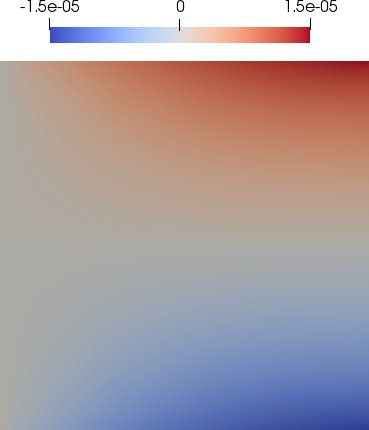
\includegraphics[width=0.45\linewidth]{data/ux.png} \hspace{1em}
    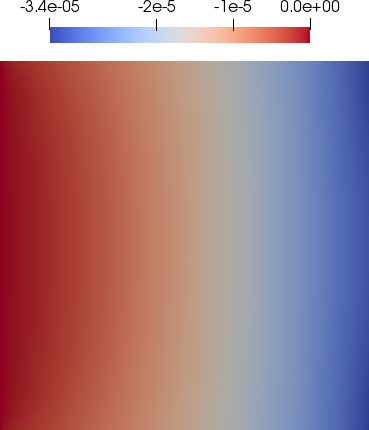
\includegraphics[width=0.45\linewidth]{data/uy.png}\\
    $\hspace{2em} u_1^{fem} \hspace{13em} u_2^{fem}$
\end{frame}

\subsection{DFM error}
\begin{frame}
    \centering
    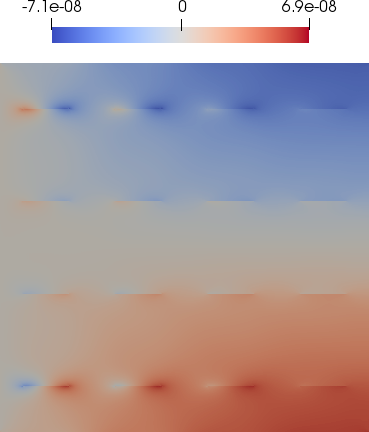
\includegraphics[width=0.45\linewidth]{data/edx.png} \hspace{1em}
    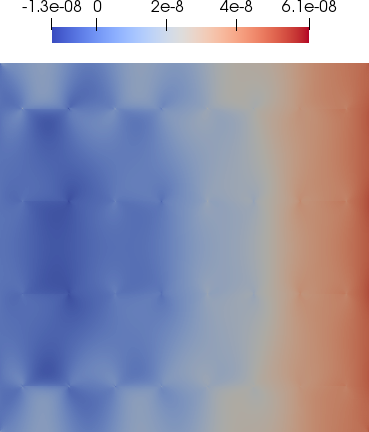
\includegraphics[width=0.45\linewidth]{data/edy.png} \\
    $u_1^{dfm}-u_1^{fem} \hspace{10em} u_2^{dfm}-u_2^{fem}$
\end{frame}

\subsection{AHM error}
\begin{frame}
    \centering
    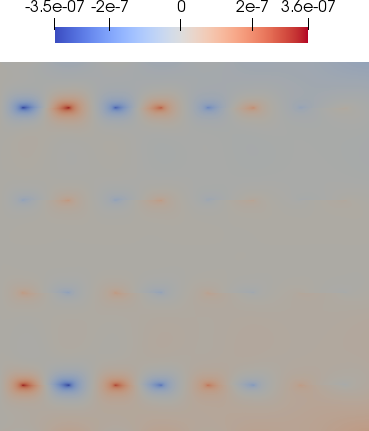
\includegraphics[width=0.45\linewidth]{data/eax.png} \hspace{1em}
    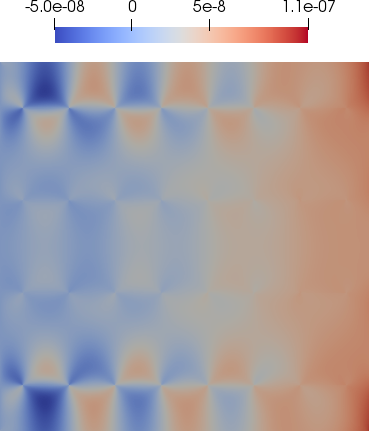
\includegraphics[width=0.45\linewidth]{data/eay.png} \\
    $u_1^{ahm}-u_1^{fem} \hspace{10em} u_2^{ahm}-u_2^{fem}$
\end{frame}

\subsection{Relative errors}
\begin{frame}
    \centering 
    DFM relative error        
    \[
        \epsilon^{dfm}_{L_\infty} = \frac{\Vert \bm{u}^{dfm} - \bm{u}^{fem} \Vert_{L_\infty}}{\Vert \bm{u}^{fem} \Vert_{L_\infty}}, \quad
    \epsilon^{dfm}_{L_2} = \frac{\Vert \bm{u}^{dfm} - \bm{u}^{fem} \Vert_{L_2}}{\Vert \bm{u}^{fem} \Vert_{L_2}},     
    \]
    \vspace{1em}

    AHM relative error
    \[
        \epsilon^{ahm}_{L_\infty} = \frac{\Vert \bm{u}^{ahm} - \bm{u}^{fem} \Vert_{L_\infty}}{\Vert \bm{u}^{fem} \Vert_{L_\infty}}, \quad
        \epsilon^{ahm}_{L_2} = \frac{\Vert \bm{u}^{ahm} - \bm{u}^{fem} \Vert_{L_2}}{\Vert \bm{u}^{fem} \Vert_{L_2}},     \]
\end{frame}

\subsection{Number of fibers in $\omega$}
\begin{frame}
    \centering
    \begin{tikzpicture}[scale=0.95]
        \begin{axis}[
            xmode=log,
            ymode=log,
            log basis x=2,
            log basis y=2,
            xlabel={$k$},
            grid=major,
            legend pos=south east,
            legend columns=2]
            \addplot[mark=square*,solid,red] table[y=edli]{data/k.txt};
            \addplot[mark=square*,solid,blue] table[y=eali]{data/k.txt};
            \addplot[mark=*,dashed,red] table[y=edl2]{data/k.txt};
            \addplot[mark=*,dashed,blue] table[y=eal2]{data/k.txt};
            \addlegendentry{$\epsilon^{dfm}_{L_\infty}$}
            \addlegendentry{$\epsilon^{ahm}_{L_\infty}$}
            \addlegendentry{$\epsilon^{dfm}_{L_2}$}
            \addlegendentry{$\epsilon^{ahm}_{L_2}$}
        \end{axis}
    \end{tikzpicture}
\end{frame}

\subsection{Thickness of fibers}
\begin{frame}
    \centering
    \begin{tikzpicture}[scale=0.95]
        \begin{axis}[
            xmode=log,
            ymode=log,
            log basis x=2,
            log basis y=2,
            xlabel={$d$},
            grid=major,
            legend pos=south east,
            legend columns=2]
            \addplot[mark=square*,solid,red] table[y=edli]{data/d.txt};
            \addplot[mark=square*,solid,blue] table[y=eali]{data/d.txt};
            \addplot[mark=*,dashed,red] table[y=edl2]{data/d.txt};
            \addplot[mark=*,dashed,blue] table[y=eal2]{data/d.txt};
            \addlegendentry{$\epsilon^{dfm}_{L_\infty}$}
            \addlegendentry{$\epsilon^{ahm}_{L_\infty}$}
            \addlegendentry{$\epsilon^{dfm}_{L_2}$}
            \addlegendentry{$\epsilon^{ahm}_{L_2}$}
        \end{axis}
    \end{tikzpicture}
\end{frame}

\subsection{Ratio of Young modulus}
\begin{frame}
    \centering
    \begin{tikzpicture}[scale=0.95]
        \begin{axis}[
            xmode=log,
            ymode=log,
            log basis x=2,
            log basis y=2,
            xlabel={$\alpha$},
            grid=major,
            legend pos=north west,
            legend columns=2]
            \addplot[mark=square*,solid,red] table[y=edli]{data/f.txt};
            \addplot[mark=square*,solid,blue] table[y=eali]{data/f.txt};
            \addplot[mark=*,dashed,red] table[y=edl2]{data/f.txt};
            \addplot[mark=*,dashed,blue] table[y=eal2]{data/f.txt};
            \addlegendentry{$\epsilon^{dfm}_{L_\infty}$}
            \addlegendentry{$\epsilon^{ahm}_{L_\infty}$}
            \addlegendentry{$\epsilon^{dfm}_{L_2}$}
            \addlegendentry{$\epsilon^{ahm}_{L_2}$}
        \end{axis}
    \end{tikzpicture}    
\end{frame}

\subsection{Number of subdomains in one direction}
\begin{frame}
    \centering
    \begin{tikzpicture}[scale=0.95]
        \begin{axis}[
            xmode=log,
            ymode=log,
            log basis x=2,
            log basis y=2,
            xlabel={$n$},
            grid=major,
            legend pos=north east,
            legend columns=2]
            \addplot[mark=square*,solid,red] table[y=edli]{data/n.txt};
            \addplot[mark=square*,solid,blue] table[y=eali]{data/n.txt};
            \addplot[mark=*,dashed,red] table[y=edl2]{data/n.txt};
            \addplot[mark=*,dashed,blue] table[y=eal2]{data/n.txt};
            \addlegendentry{$\epsilon^{dfm}_{L_\infty}$}
            \addlegendentry{$\epsilon^{ahm}_{L_\infty}$}
            \addlegendentry{$\epsilon^{dfm}_{L_2}$}
            \addlegendentry{$\epsilon^{ahm}_{L_2}$}
        \end{axis}
    \end{tikzpicture}
\end{frame}

\subsection{Grid step ($d=1/64, l=1/8$)}
\begin{frame}
\centering
\begin{tikzpicture}[scale=1]
    \begin{axis}[
        xmode=log,
        ymode=log,
        log basis x=2,
        log basis y=2,
        xlabel={$h$},
        grid=major,
        legend style={at={(0.03,0.57)},anchor=north west},
        legend columns=2]
        \addplot[mark=square*,solid,red] table[y=edli]{data/h.txt};
        \addplot[mark=square*,solid,blue] table[y=eali]{data/h.txt};
        \addplot[mark=*,dashed,red] table[y=edl2]{data/h.txt};
        \addplot[mark=*,dashed,blue] table[y=eal2]{data/h.txt};
        \addlegendentry{$\epsilon^{dfm}_{L_\infty}$}
        \addlegendentry{$\epsilon^{ahm}_{L_\infty}$}
        \addlegendentry{$\epsilon^{dfm}_{L_2}$}
        \addlegendentry{$\epsilon^{ahm}_{L_2}$}
    \end{axis}
\end{tikzpicture}
\end{frame}

\section{Conclusion}
\subsection{Conclusion}
\begin{frame}
    \begin{itemize}
        \item DFM comparing to AHM showed better accuracy for a large ratio of Young modulus
        \item DFM is more convenient for thick fibers
        \item AHM solution is better for a large number of equal subdomains
        \item Using DFM we can solve on more coarse meshes
    \end{itemize}
 \end{frame}

\subsection{Thank you}
\begin{frame}
    \centering
    Thank you for your attention!
\end{frame}

\end{document}
